\section[Desenvolvimento do Projeto]{Desenvolvimento do Projeto}

\subsection{Repositório do Código Fonte do Projeto}

Adotamos o GitHub \cite{github-docs} como plataforma principal de
versionamento. Os repositórios do GitLab \cite{gitlab-docs} da AGES recebiam
as alterações por espelhamento. Os \textit{workflows} do GitHub Actions
\cite{github-actions-docs} replicavam as \textit{branches main} e
\textit{develop}, além das \textit{tags}, mantendo uma cópia sincronizada
do código na plataforma da disciplina.

A \textit{branch main} reunia a versão estável, e a \textit{develop}, as
funcionalidades em integração. Desenvolvíamos as tarefas em \textit{branches}
próprias. No \textit{backend}, um \textit{hook} local bloqueava
\textit{commits} em ramos que não seguissem a convenção
\textit{tidXXX/descricao-da-tarefa}. O identificador da tarefa no nome da
\textit{branch} ajudava a relacionar as alterações à demanda durante a revisão
dos \acp{pr}.

O \textit{backend} executava testes e verificações de estilo e formatação com
Ruff \cite{ruff-docs} durante a revisão dos \acp{pr}. Os dois repositórios
também tinham instruções de execução e de organização do código para orientar
a configuração do ambiente pelos integrantes da equipe.

Repositório \textit{backend}:

{\footnotesize\urlstyle{same}\urlref{https://tools.ages.pucrs.br/2026-2/2jk-4jk/hangy/hangy-backend}}

Repositório \textit{frontend}:

{\footnotesize\urlstyle{same}\urlref{https://tools.ages.pucrs.br/2026-2/2jk-4jk/hangy/hangy-frontend}}

\subsection{Banco de Dados Utilizado}

Usamos PostgreSQL \cite{postgresql-docs} com a extensão PostGIS
\cite{postgis-docs}. Escolhemos um banco relacional pelas relações entre
usuários, eventos, categorias, participações e notificações. As localizações
dos eventos e dos perfis de negócio eram armazenadas com o tipo
\textit{geography(Point,4326)}, que permitia trabalhar com a proximidade
geográfica. Durante o desenvolvimento, executávamos o banco em contêiner e
aplicávamos as migrações nesse ambiente.

A entidade \mbox{\textit{USER}} armazenava os dados de autenticação e o tipo
de conta. Usamos \mbox{\textit{PERSON\_PROFILE}} para os perfis pessoais e
\mbox{\textit{BUSINESS\_PROFILE}} para os dados das organizações. Cada evento
era vinculado ao seu criador. As tabelas \mbox{\textit{EVENT\_TAG}} e
\mbox{\textit{EVENT\_PARTICIPANT}} associavam os eventos a suas categorias e
participantes. O modelo também previa conexões e seguidores entre usuários,
experiências de eventos, denúncias e notificações.

Usamos \ac{uuid} nas chaves primárias e estrangeiras. Os tipos enumerados
delimitavam os valores aceitos para privacidade e situação dos eventos,
participações, notificações e denúncias. Nas principais entidades, campos de
criação, atualização e exclusão lógica registravam o ciclo de vida dos dados.

\par\addvspace{0.3\baselineskip}
\noindent\begin{minipage}{\linewidth}
\setlength{\parindent}{1.25cm}
\setlength{\intextsep}{4pt}
A Figura \ref{fig:hangy-database} apresenta o modelo de dados.

\begin{figure}[H]
    \centering
    \small
    \caption{Modelo de dados do projeto Hangy}
    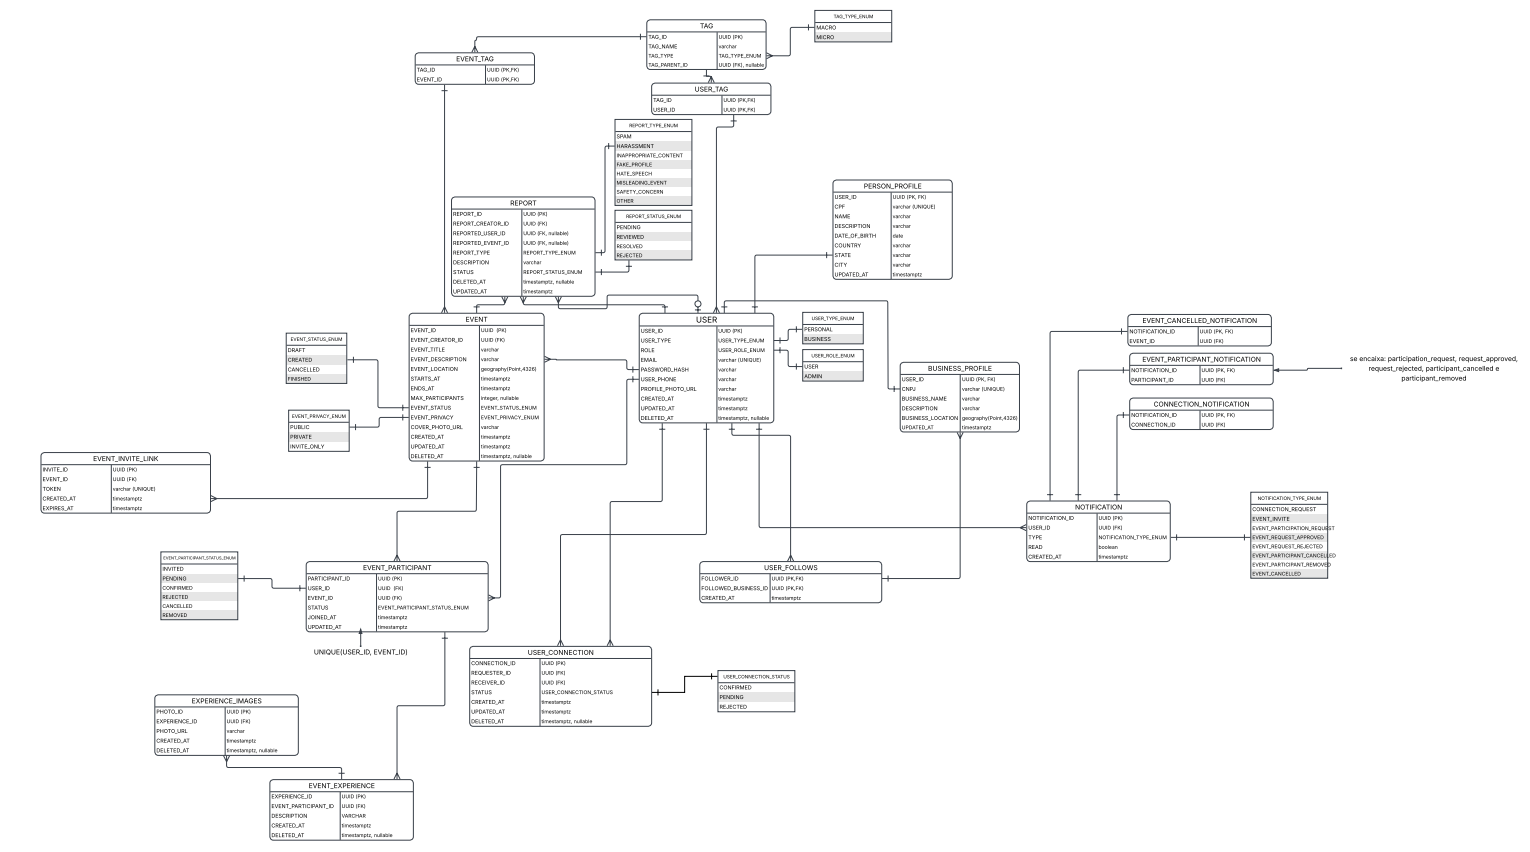
\includegraphics[width=\linewidth]{conteudo//5 - ages IV//conteudo//figures/hangy-db.png}
    \legend{Fonte: Wiki do projeto}
    \label{fig:hangy-database}
\end{figure}
\end{minipage}
\par\addvspace{0.3\baselineskip}

{\footnotesize\urlstyle{same}\urlref{https://tools.ages.pucrs.br/2026-2/2jk-4jk/hangy/wiki/-/wikis/database}}

\subsection{Arquitetura Utilizada}

\par\addvspace{0.3\baselineskip}
\noindent\begin{minipage}{\linewidth}
\setlength{\parindent}{1.25cm}
\setlength{\intextsep}{4pt}
A Figura \ref{fig:hangy-architecture-general} apresenta a comunicação entre
o aplicativo e a \ac{api}. O aplicativo móvel foi desenvolvido com React
Native, Expo e TypeScript. A \ac{api}, em FastAPI, recebia as requisições
\ac{http} e tratava as regras de negócio, a autenticação e o acesso aos dados.
O aplicativo cuidava das telas e da navegação.

\begin{figure}[H]
    \centering
    \small
    \caption{Visão geral da arquitetura do Hangy}
    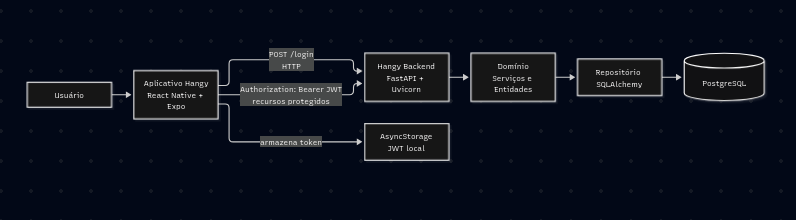
\includegraphics[width=\linewidth]{conteudo//5 - ages IV//conteudo//figures/hangy-architecture-general.png}
    \legend{Fonte: Wiki do projeto}
    \label{fig:hangy-architecture-general}
\end{figure}
\end{minipage}
\par\addvspace{0.3\baselineskip}

No \textit{backend}, seguimos uma arquitetura em camadas inspirada na
\textit{Clean Architecture} \cite{martin-clean-architecture}. A camada
\textit{presentation} recebia as requisições e definia os contratos de entrada
e saída por meio de \acp{dto}. A camada \textit{domain} reunia as entidades,
enumerações e serviços com as regras de negócio. A camada
\textit{infrastructure} continha as sessões, os modelos SQLAlchemy e os
repositórios de acesso ao PostgreSQL. Os serviços dependiam de contratos de
repositório, enquanto os detalhes de persistência ficavam nas implementações
desses contratos.

No \textit{frontend}, as telas e os \textit{layouts} de navegação ficavam em
\textit{src/app}, conforme as convenções do Expo Router. Componentes
reutilizáveis, \textit{hooks}, constantes e utilitários tinham diretórios
próprios dentro de \textit{src/}. Essa organização separava a interface da
lógica de cada tela e centralizava os elementos do \textit{design system}.

A comunicação seguia o padrão \ac{rest}. No \textit{login}, o aplicativo
enviava as credenciais à \ac{api}, recebia um \ac{jwt} e o guardava no
AsyncStorage \cite{asyncstorage-docs}. Depois, enviava o \textit{token} no
cabeçalho \textit{Authorization: Bearer} das requisições protegidas. O
\textit{backend} verificava a assinatura e a expiração antes de permitir o
acesso. Armazenávamos as senhas como \textit{hashes} Argon2
\cite{argon2-reference}, e as mudanças de estrutura do banco eram
versionadas com Alembic.

Os \textit{mappers} convertiam as entradas, e os \textit{assemblers}
montavam as respostas. O FastAPI injetava os repositórios nos serviços.

{\footnotesize\urlstyle{same}\urlref{https://tools.ages.pucrs.br/2026-2/2jk-4jk/hangy/wiki/-/wikis/arquitetura}}

\subsection{Protótipos das Telas Desenvolvidas}

\par\addvspace{0.3\baselineskip}
\noindent\begin{minipage}{\linewidth}
\setlength{\parindent}{1.25cm}
\setlength{\intextsep}{4pt}
A Figura \ref{fig:hangy-mockup-home} mostra a tela inicial, que agrupava os
eventos por interesses, como bem-estar, esportes e cafeteria. Os cartões
apresentavam visibilidade, data, local e categorias. A barra inferior dava
acesso às principais áreas do aplicativo.

\begin{figure}[H]
    \centering
    \small
    \caption{Tela inicial do aplicativo Hangy}
    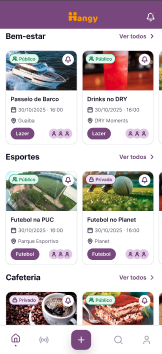
\includegraphics[height=0.33\textheight]{conteudo//5 - ages IV//conteudo//figures/hangy-mockup-home.png}
    \legend{Fonte: Figma do projeto}
    \label{fig:hangy-mockup-home}
\end{figure}
\end{minipage}
\par\addvspace{0.3\baselineskip}

\par\addvspace{0.3\baselineskip}
\noindent\begin{minipage}{\linewidth}
\setlength{\parindent}{1.25cm}
\setlength{\intextsep}{4pt}
A Figura \ref{fig:hangy-mockup-event-flows} apresenta as telas de detalhes e
criação de evento. A primeira exibia capa, categorias, data, local, descrição
e a ação disponível ao usuário. A segunda orientava o preenchimento do nome,
descrição e imagem de capa, além da escolha de \textit{tags} agrupadas por
categorias.

\begin{figure}[H]
    \centering
    \small
    \caption{Telas de detalhes e criação de evento do Hangy}
    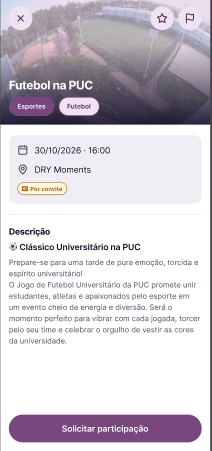
\includegraphics[height=0.33\textheight]{conteudo//5 - ages IV//conteudo//figures/hangy-mockup-event-details.png}
    \hfill
    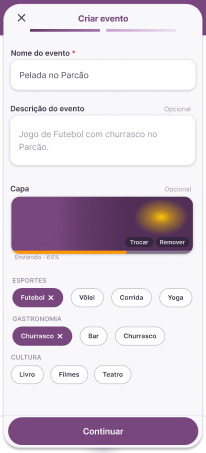
\includegraphics[height=0.33\textheight]{conteudo//5 - ages IV//conteudo//figures/hangy-mockup-create-event.png}
    \legend{Fonte: Figma do projeto}
    \label{fig:hangy-mockup-event-flows}
\end{figure}
\end{minipage}
\par\addvspace{0.3\baselineskip}

{\footnotesize\urlstyle{same}\urlref{https://tools.ages.pucrs.br/2026-2/2jk-4jk/hangy/wiki/-/wikis/mockups}}

\subsection{Tecnologias Utilizadas}

Mantivemos tecnologias que já havíamos utilizado no VanGO, como Python,
FastAPI, TypeScript, React Native e Expo. No \textit{backend}, usamos Python
3.14 \cite{python-docs} e FastAPI \cite{fastapi-docs}, que disponibilizava a
documentação da \ac{api} pela especificação OpenAPI. O Uvicorn
\cite{uvicorn-docs} executava a aplicação no padrão \ac{asgi}, e o Pydantic
\cite{pydantic-docs} validava os dados recebidos.

O SQLAlchemy \cite{sqlalchemy-docs} fazia o mapeamento dos dados para o
PostgreSQL. O PostGIS acrescentava os recursos geoespaciais, e o Alembic
\cite{alembic-docs} versionava as migrações. Para a autenticação, utilizamos
\ac{jwt} \cite{jwt-rfc}, com PyJWT \cite{pyjwt-docs} para gerar e validar os
\textit{tokens} e \textit{pwdlib} \cite{pwdlib-docs} com Argon2 para calcular
os \textit{hashes} das senhas.

Executávamos os testes automatizados com Pytest \cite{pytest-docs} e HTTPX
\cite{httpx-docs}. O Ruff fazia a análise e a formatação do código. Docker,
Docker Compose e Dev Containers \cite{docker-docs} organizavam a execução
local da \ac{api}, do PostgreSQL e das ferramentas de desenvolvimento.

No \textit{frontend}, usamos TypeScript \cite{typescript-docs}, React Native
\cite{react-native-docs} e Expo \cite{expo-docs} para desenvolver um aplicativo
compatível com Android, iOS e \textit{web}. O Expo Router organizava a
navegação por arquivos, e o AsyncStorage mantinha o \ac{jwt} localmente.
Bibliotecas do Expo davam acesso a arquivos, imagens, seleção de mídia e
ligações externas. Os ícones eram do Lucide React Native \cite{lucide-docs}.
